\chapter[METHODOLOGY]{Methodology}\label{ch:III}

This chapter describes how the application was developed and evaluated. As shown
in Figure~\ref{fig:3.1}, the study proceeded in five phases: requirements
gathering, analysis and design, implementation, deployment, and user testing and
evaluation.

\begin{figure}[htbp]
\centering
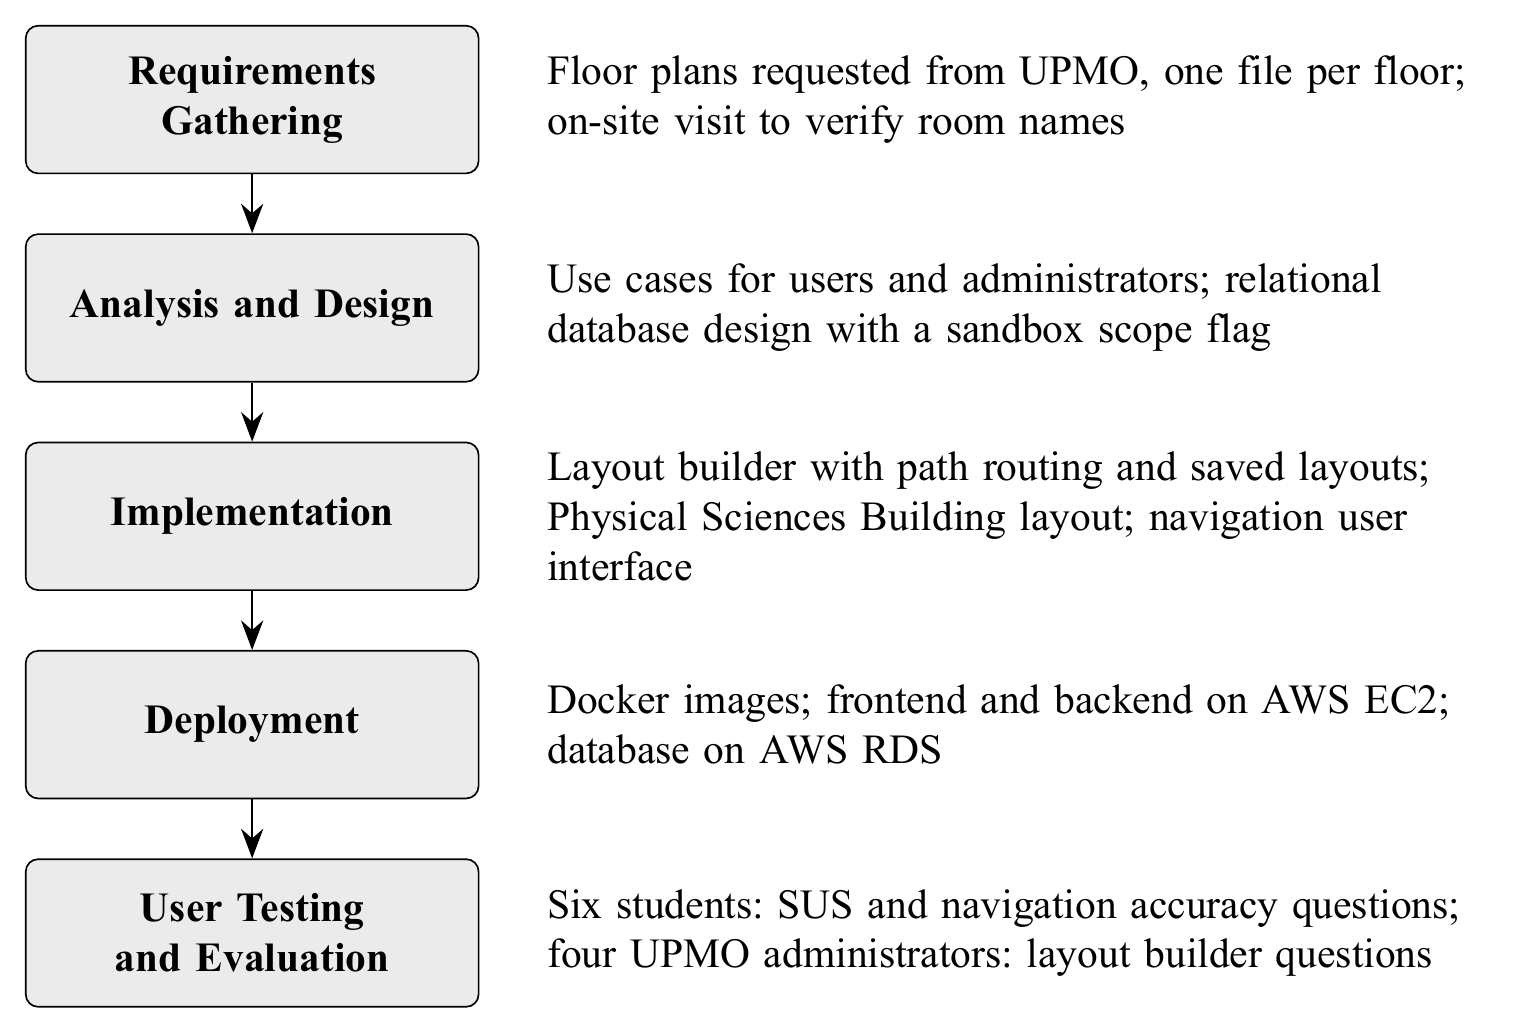
\includegraphics[width=5.10in]{figures/fig-3-1.png}
\caption{Phases of the study}\label{fig:3.1}
\end{figure}

\section{Requirements Gathering}\label{sec:3.1}

In order to retrieve the correct layout of the Physical Sciences Building, an
email was sent to the University Planning and Maintenance Office (UPMO) to
request the building's floor plans. A 2D layout of the building was provided,
separated into three files, with each file mapping out an entire floor.

For the labeling of the rooms, a physical visit inside the building was
conducted to cross-examine the accuracy of the floor plan against the actual
rooms, including the name of each room. After development of the application,
another email was sent to UPMO to request user testing. Administrators from
their office were asked to participate in testing the layout builder feature of
the application.

\section{Analysis and Design}\label{sec:3.2}

Figure~\ref{fig:3.2} shows the use-case diagram for the indoor navigation web
application. Two actor roles were identified: users and administrators, each
with distinct capabilities within the system. Users were able to search for
rooms, select an origin and destination, and view the generated navigation
route. Administrators, in addition to having access to navigation features, were
able to create, edit, and publish floor layouts through the layout builder,
giving them control over the data that powered the navigation feature for all
users.

\begin{figure}[htbp]
\centering
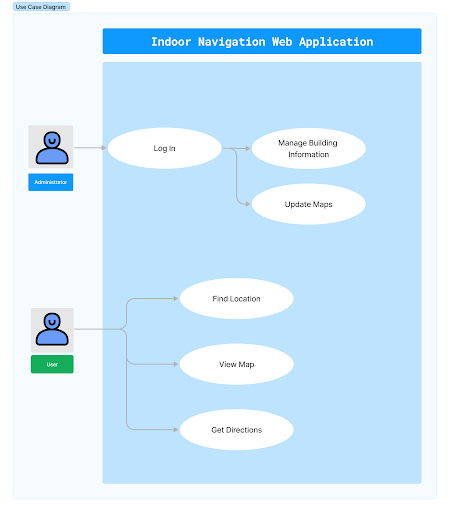
\includegraphics[width=3.90in]{figures/fig-3-2.png}
\caption{Use-case diagram of the indoor navigation web application}\label{fig:3.2}
\end{figure}

Based on these use cases, the system was designed around a relational database
structure using MariaDB. During backend startup, the database service connected
to the database and verified that the required schemas were present before the
application became available. A scope flag was incorporated within the relevant
tables to separate live, published records from sandbox records, allowing
administrators to edit and test layout changes without affecting the version
currently used for navigation.

Figure~\ref{fig:3.3} shows the Entity Relationship Diagram (ERD) of the
application database. The login\_accounts table stores the administrator
accounts used to access the layout builder. The draft\_map\_layouts table stores
unpublished layout drafts, and each draft may be published as entries in the
map\_layouts table, which holds the published layouts together with a flag
marking the current version. Each published layout may in turn be cached by
entries in the navigation\_graph\_caches table, which stores the navigation
graph computed from that layout. The buildings, floors, rooms, and associated
navigation data are held in the layout\_json and graph\_json columns, while the
is\_sandbox column serves as the scope flag that separates sandbox records from
live records.

\begin{figure}[htbp]
\centering
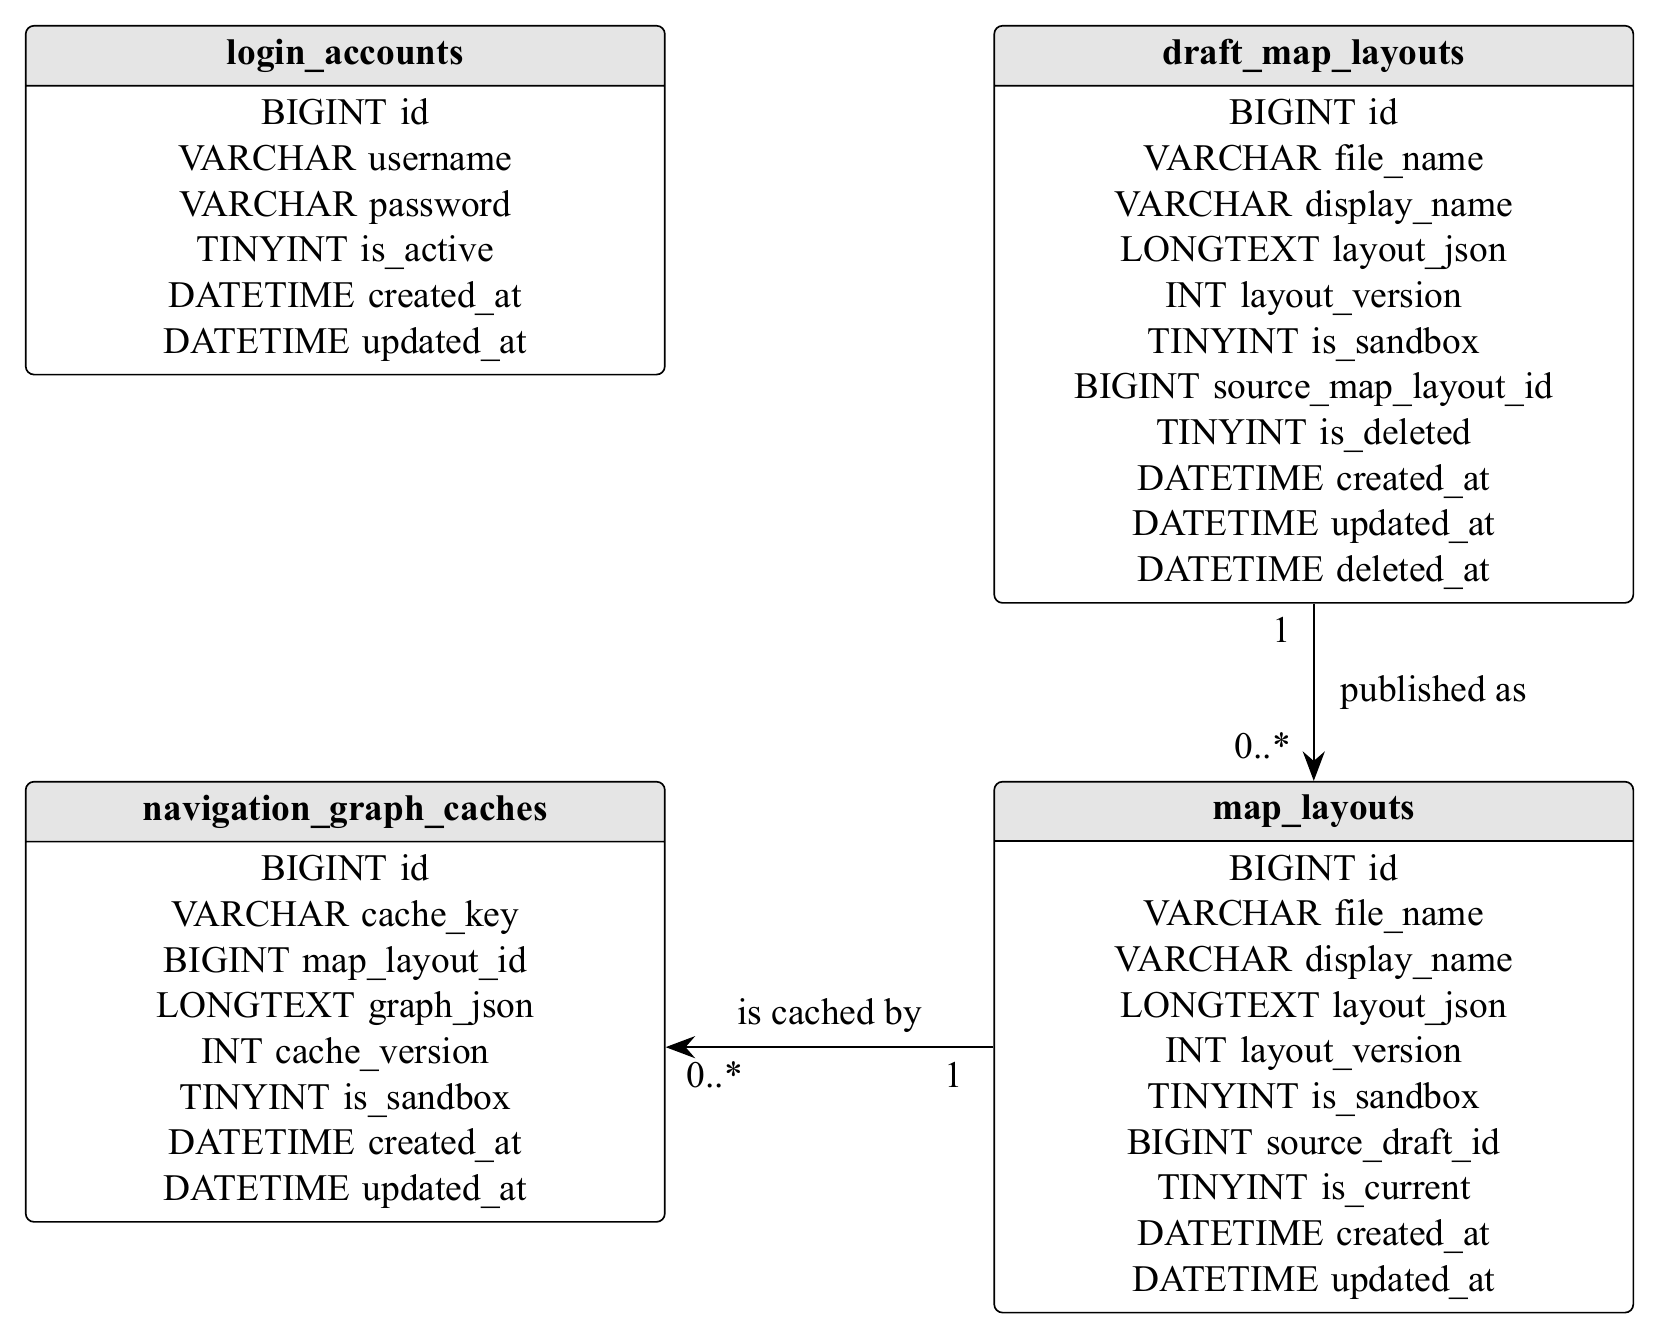
\includegraphics[width=5.53in]{figures/fig-3-3.png}
\caption{Entity relationship diagram of the application database}\label{fig:3.3}
\end{figure}

\section{Development Tools}\label{sec:3.3}

A laptop with the specifications listed in Table~\ref{tab:3.1} was used to
develop the indoor navigation web application.

\begin{table}[htbp]
\centering
\singlespacing
\caption{Hardware specifications of the development machine}\label{tab:3.1}
\renewcommand{\arraystretch}{1.15}
\begin{tabular}{ll}
\toprule
\textbf{Component} & \textbf{Specification} \\
\midrule
Operating system & Windows 11, 64-bit \\
Processor & Intel® Core™ i5-8250U, 1.6 GHz \\
Graphics card & NVIDIA GeForce GTX 1050 \\
Memory & 20 GB DDR4, 2800 MHz \\
\bottomrule
\end{tabular}
\end{table}

The software development tools listed in Table~\ref{tab:3.2} were used in the
development of the application.

\begin{table}[htbp]
\centering
\singlespacing
\caption{Software development tools}\label{tab:3.2}
\renewcommand{\arraystretch}{1.15}
\begin{tabularx}{\linewidth}{lX}
\toprule
\textbf{Tool} & \textbf{Description} \\
\midrule
Python & An interpreted, object-oriented, high-level programming language, used to build the backend component of the application \\
MariaDB & An open-source relational database management system \\
React & An open-source front-end JavaScript library, used to build the frontend component of the application \\
Visual Studio Code & A source-code editor used for developing the application \\
\bottomrule
\end{tabularx}
\end{table}

\section{Implementation}\label{sec:3.4}

The application was built first with the layout builder features in mind. The
goal was to create a working map layout with the integration of path routing and
a persistence state to save layouts. A layout of the Physical Sciences Building
was then created using the layout builder, guided by the floor plan provided by
UPMO. After that, focus shifted to the user interface, allowing users to select
between different rooms. Finally, once the application was built, it was
deployed on AWS to test the application's stability outside the local
development environment.

\section{Deployment}\label{sec:3.5}

The application was deployed on Amazon Web Services (AWS). The following AWS
services were used:

\begin{itemize}
\item
  \textbf{Elastic Compute Cloud (EC2)} -- an EC2 instance was created to
  configure and run both the frontend and the backend services.
\item
  \textbf{Relational Database Service (RDS)} -- a managed cloud database that
  handled the storage of data and database operations.
\end{itemize}

The application's backend and frontend were each packaged as separate Docker
images. This containerization approach supported a more consistent and
repeatable deployment process across the development lifecycle, since the same
image built and tested locally could be deployed to the cloud without
modification. Both containers run on the same AWS EC2 instance and communicate
through a shared Docker network. The frontend container serves the built React
application through an nginx web server, which makes the application publicly
accessible via a web URL and forwards the application's API requests to the
backend container. The backend container runs the Python service, which
processes these requests and connects to an AWS RDS instance that is responsible
for persisting and retrieving application data. Figure~\ref{fig:3.4} summarizes
this deployment architecture.

\begin{figure}[htbp]
\centering
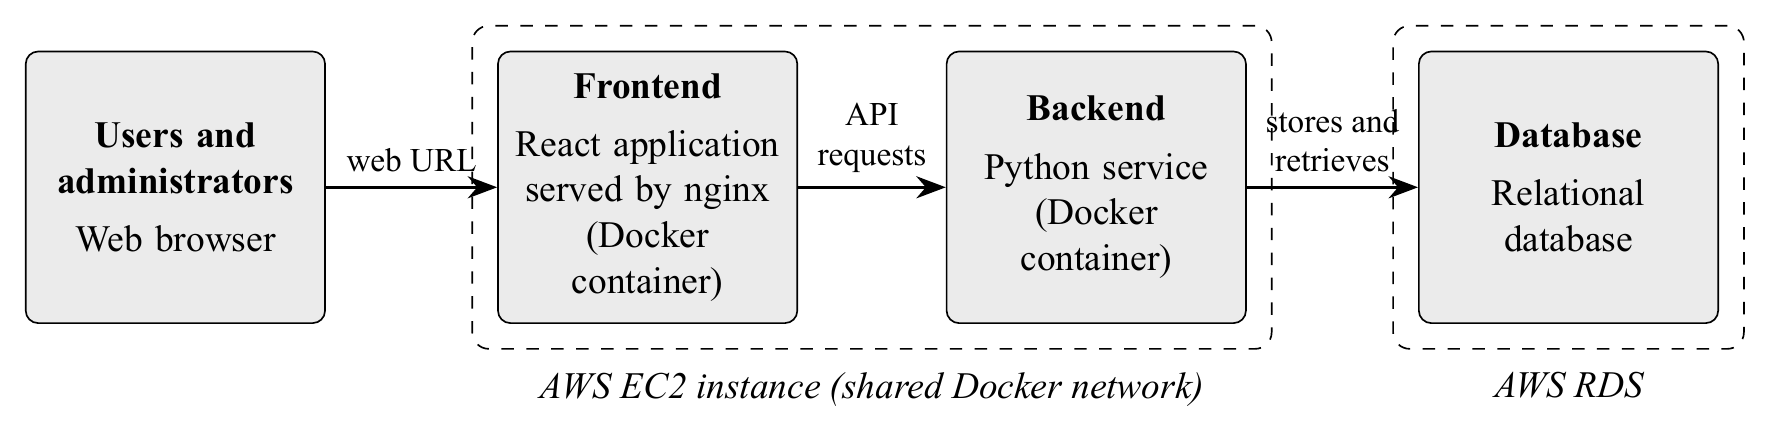
\includegraphics[width=5.90in]{figures/fig-3-4.png}
\caption{Deployment architecture of the application}\label{fig:3.4}
\end{figure}

\section{User Testing and Evaluation}\label{sec:3.6}

\subsection{Participants}\label{sec:3.6.1}

User testing was conducted with two participant groups: regular users and
building administrators. A total of ten (10) respondents took part: four (4)
building administrators from the University Planning and Maintenance Office
(UPMO) and six (6) students of the University of the Philippines Los Baños.

\subsection{Procedure}\label{sec:3.6.2}

For building administrators, the focus of testing was the map layout builder
feature, specifically whether the tools for the map layouts functioned correctly
and were practical to use. They logged in to the system, accessed the layout
builder, and tested the available editing functions, such as adding, modifying,
saving, and publishing map elements. They then verified whether the published
changes were correctly reflected in the navigation interface.

For regular users, the focus of testing was navigation accuracy, particularly
whether the application could correctly guide them from a selected origin to a
specified destination within the building and whether the displayed route
matched the actual path.

A live demonstration of the application was conducted online via Zoom, with
separate sessions held for regular users and building administrators. Questions
related to application features were accommodated during this period, and
respondents were then asked to answer a Google Form containing questions related
to system usability and navigation accuracy. A one-week testing period was given
so that all users would have ample time to explore and use the features of the
application.

\subsection{Evaluation Instruments}\label{sec:3.6.3}
% NOTE: the Word file has a review comment on this heading: "Verify To review"

To quantify the usability of the web application, the System Usability Scale
(SUS)~\cite{ref20} was used. This is a reliable tool for measuring the usability
of various systems and services. The SUS provides a set of ten statements
(Appendix A), each rated on a five-point Likert scale ranging from ``Strongly
disagree'' (1) to ``Strongly agree'' (5). This scale is designed to evaluate a
broad range of interactive products by deriving a single usability score that
reflects a composite measure of the overall effectiveness, efficiency, and
satisfaction with the system.

Following the standard SUS scoring procedure~\cite{ref20}, each odd-numbered
(positively worded) statement contributes its response minus one, and each
even-numbered (negatively worded) statement contributes five minus its response.
The ten contributions are summed and multiplied by 2.5, which yields a score
from 0 to 100:

\begin{equation}
\label{eq:3.1}
SUS = 2.5\left\lbrack \sum_{i \in \{ 1,3,5,7,9\}}^{}\left( x_{i} - 1 \right) + \sum_{i \in \{ 2,4,6,8,10\}}^{}\left( 5 - x_{i} \right) \right\rbrack
\end{equation}

\noindent where \emph{x}\textsubscript{i} is the response to statement \emph{i}.
The resulting scores were interpreted using the Sauro--Lewis curved grading
scale~\cite{ref21}, which ranks a SUS score against the scores of hundreds of
other systems, together with the adjective ratings of Bangor et
al.~\cite{ref22}, as combined by Sauro~\cite{ref23}. Table~\ref{tab:3.3} shows
the resulting interpretation, in which the average SUS score of 68 corresponds
to a grade of C.

\begin{table}[htbp]
\centering
\singlespacing
\caption{Interpretation of SUS scores}\label{tab:3.3}
\renewcommand{\arraystretch}{1.15}
\begin{tabular}{ccl}
\toprule
\textbf{SUS score} & \textbf{Percentile range} & \textbf{Adjective rating} \\
\midrule
84.1--100.0 & 96--100 & Best Imaginable \\
80.8--84.0 & 90--95 & Excellent \\
71.1--80.7 & 60--89 & Good \\
51.7--71.0 & 15--59 & OK \\
25.1--51.6 & 2--14 & Poor \\
0.0--25.0 & 0--1.9 & Worst Imaginable \\
\bottomrule
\end{tabular}
\par\vspace{4pt}
{\footnotesize\raggedright\setlength{\parindent}{0pt}Source: Sauro~\cite{ref23}; grades and percentile ranges from the Sauro--Lewis curved grading scale~\cite{ref21}.\par}
\end{table}

To evaluate navigation accuracy, a qualitative testing phase was conducted.
After completing the assigned navigation tasks, the regular users answered a set
of six open-ended questions (Appendix B) based on their experience using the
application. The responses were analyzed to determine whether the application
was capable of providing accurate and understandable indoor navigation guidance.
The building administrators answered a separate set of seven open-ended
questions about the layout builder (Appendix C).
